%%%%%%%% ICML 2024 EXAMPLE LATEX SUBMISSION FILE %%%%%%%%%%%%%%%%%

\documentclass{article}

% Recommended, but optional, packages for figures and better typesetting:
\usepackage{microtype}
\usepackage{graphicx}
\usepackage{svg}
\usepackage{natbib}
\usepackage{booktabs} % for professional tables
\usepackage{tikz}
\usetikzlibrary{arrows.meta, shapes.geometric, calc}
% hyperref makes hyperlinks in the resulting PDF.
% If your build breaks (sometimes temporarily if a hyperlink spans a page)
% please comment out the following usepackage line and replace
% \usepackage{icml2024} with \usepackage[nohyperref]{icml2024} above.
\usepackage{hyperref}


% Attempt to make hyperref and algorithmic work together better:
\newcommand{\theHalgorithm}{\arabic{algorithm}}

% Use the following line for the initial blind version submitted for review:
\usepackage{icml2024}

% If accepted, instead use the following line for the camera-ready submission:
%\usepackage[accepted]{icml2024}

% For theorems and such
\usepackage{amsmath}
\usepackage{amssymb}
\usepackage{mathtools}
\usepackage{amsthm}

% if you use cleveref..
\usepackage[capitalize,noabbrev]{cleveref}

%%%%%%%%%%%%%%%%%%%%%%%%%%%%%%%%
% THEOREMS
%%%%%%%%%%%%%%%%%%%%%%%%%%%%%%%%
\theoremstyle{plain}
\newtheorem{theorem}{Theorem}[section]
\newtheorem{proposition}[theorem]{Proposition}
\newtheorem{lemma}[theorem]{Lemma}
\newtheorem{corollary}[theorem]{Corollary}
\theoremstyle{definition}
\newtheorem{definition}[theorem]{Definition}
\newtheorem{assumption}[theorem]{Assumption}
\theoremstyle{remark}
\newtheorem{remark}[theorem]{Remark}

% Todonotes is useful during development; simply uncomment the next line
%    and comment out the line below the next line to turn off comments
%\usepackage[disable,textsize=tiny]{todonotes}
\usepackage[textsize=tiny]{todonotes}


% The \icmltitle you define below is probably too long as a header.
% Therefore, a short form for the running title is supplied here:
\icmltitlerunning{Displacement-Sparse Neural Optimal Transport}

\begin{document}

\twocolumn[
\icmltitle{Displacement-Sparse Neural Optimal Transport}

% It is OKAY to include author information, even for blind
% submissions: the style file will automatically remove it for you
% unless you've provided the [accepted] option to the icml2024
% package.

% List of affiliations: The first argument should be a (short)
% identifier you will use later to specify author affiliations
% Academic affiliations should list Department, University, City, Region, Country
% Industry affiliations should list Company, City, Region, Country

% You can specify symbols, otherwise they are numbered in order.
% Ideally, you should not use this facility. Affiliations will be numbered
% in order of appearance and this is the preferred way.

\begin{icmlauthorlist}
\icmlauthor{Peter Chen}{cms,ids}
\icmlauthor{Yue Xie}{ids}
\icmlauthor{Qingpeng Zhang}{ids,hkus}

%\icmlauthor{}{sch}
%\icmlauthor{}{sch}
\end{icmlauthorlist}

\icmlaffiliation{cms}{Department of Mathematics, Columbia University, New York, USA}
\icmlaffiliation{ids}{HKU Musketeers Foundation Institute of Data Science, Hong Kong}
\icmlaffiliation{hkus}{HKU Shanghai Intelligent Computing Research Center, Shanghai, China}

\icmlcorrespondingauthor{Yue Xie}{yxie@hku.hk}
\icmlcorrespondingauthor{Qingpeng Zhang}{qpzhang@hku.hk}

% You may provide any keywords that you
% find helpful for describing your paper; these are used to populate
% the "keywords" metadata in the PDF but will not be shown in the document
\icmlkeywords{Machine Learning}

\vskip 0.3in
]

% this must go after the closing bracket ] following \twocolumn[ ...

% This command actually creates the footnote in the first column
% listing the affiliations and the copyright notice.
% The command takes one argument, which is text to display at the start of the footnote.
% The \icmlEqualContribution command is standard text for equal contribution.
% Remove it (just {}) if you do not need this facility.

%\printAffiliationsAndNotice{}  % leave blank if no need to mention equal contribution
\printAffiliationsAndNotice{\icmlEqualContribution} % otherwise use the standard text.

\begin{abstract}
Optimal Transport (OT) theory seeks to determine the map $T:X \to Y$ that transports a source measure \( P \) to a target measure \( Q \), minimizing the cost \( c(\mathbf{x}, T(\mathbf{x})) \) between \(\mathbf{x}\) and its image \( T(\mathbf{x}) \). Building upon the Input Convex Neural Network OT solver \cite{Makkuva20, Amos17} and incorporating the concept of displacement-sparse maps \cite{Cuturi23}, we introduce a sparsity penalty into the minimax Wasserstein formulation, promote sparsity in displacement vectors \(\Delta(\mathbf{x}) := T(\mathbf{x}) - \mathbf{x}\), and enhance the interpretability of the resulting map. However, increasing sparsity often reduces feasibility, causing \( T_{\#}(P) \) to deviate more significantly from the target measure. In low-dimensional settings, we propose a heuristic framework to balance the trade-off between sparsity and feasibility by dynamically adjusting the sparsity intensity parameter during training. For high-dimensional settings, we directly constrain the dimensionality of displacement vectors by enforcing \(\dim(\Delta(\mathbf{x})) \leq l\), where \( l < d \) for \( X \subseteq \mathbb{R}^d \). Among maps satisfying this constraint, we aim to identify the most feasible one. This goal can be effectively achieved by adapting our low-dimensional heuristic framework without resorting to dimensionality reduction. We validate our method on both synthesized sc-RNA and real 4i cell perturbation datasets, demonstrating improvements over existing methods.
\end{abstract}

\section{Introduction}
Optimal transport (OT) aims to find a map \( T \) that efficiently transfers mass from one measure to another under the ground-truth cost. This technique has been applied in various machine-learning-based single-cell biology studies, as demonstrated in \cite{Huizing22, Zhang21, Dem22, Sch19, Bunne23}. Compared to traditional methods of solving OT, such as Sinkhorn's algorithm \cite{Cut13}, recent studies in single-cell biology have increasingly utilized Neural Optimal Transport (Neural OT) solvers. These solvers efficiently scale OT to large-scale and high-dimensional problems using continuous methods \cite{Korotin21}. For instance, CellOT \cite{Bunne23} addresses cell perturbation response by leveraging Neural OT, implemented via the Input Convex Neural Network (ICNN) framework.

While Neural OT solvers can produce feasible maps, the lack of sparsity in the displacement vector reduces their interpretability, often resulting in overly complex OT maps that involve all dimensions (features). To address the similar issue in the Sinkhorn-solved map, \citet{Cuturi23} introduced the concept of displacement-sparse maps. These maps are more interpretable with lower-dimensional displacement while preserving their applicability in the original space without relying on dimensionality reduction techniques. Inspired by this work, we extend similar sparsity-promoting features to Neural OT solvers, specifically the Neural OT solver implemented via ICNN \cite{Makkuva20} (referred to as ``ICNN OT" in the following discussion).

Building on the minimax formulation of the Kantorovich dual problem used in ICNN OT, we incorporate sparsity penalties into the framework. This builds on the re-parameterization of the dual potentials \(f\) and \(g\) as convex functions, which can be efficiently learned through ICNN training. The sparsity penalty is inspired by the \citet{Cuturi23}'s sparsity-induced transportation cost function, which is defined as \(c(\mathbf{x}, \mathbf{y}) = \frac{1}{2} \|\mathbf{x} - \mathbf{y}\|_2^2 + \lambda \cdot \tau\). Here, \(\tau\) serves as a sparsity regulator, and \(\lambda\) controls the intensity of the sparsity-inducing.

\begin{figure*}[t]
    \centering
    \includegraphics[width=0.95\textwidth]{Figure1.pdf} % Ensure the path to Figure1.png is correct
    \vspace{-0.5em} % Adjust space between legend and caption
    \caption{OT maps induced by various sparsity penalties $\tau(\cdot)$ at different intensity levels $\lambda$. The first column presents the maps produced by ICNN OT and the traditional Sinkhorn algorithm implemented using \texttt{OTT-JAX} \cite{cuturi2022ottjax}, both without sparsity penalties. The subsequent columns illustrate maps learned via ICNN with sparsity penalties, specifically $\ell_{1}$ and $\tau_{\text{stvs}}$: the top row corresponds to maps trained with lower sparsity intensities, while the bottom row represents maps trained with higher sparsity intensities. Randomly selected points from the source distribution are used to showcase the displacement vectors (arrows) learned through OT. Example of aggregate results are shown in \hyperref[f2]{Figure 2}.}
    \label{f1}
\end{figure*}

However, inducing sparsity in OT maps comes with a trade-off: as the sparsity level increases, the accuracy of the map's feasibility decreases, which means that the source measure cannot be effectively transported to the target measure. This effect is evident in \hyperref[f2]{Figure 2}, where at higher sparsity intensity level, less points can be effectively transported to the target location, and displacement vectors are becoming shorter due to the stronger sparsity penalty. To tackle this issue, we create a dynamic framework to adjust the sparsity intensity, offering two models to solve OT tasks in both low-dimensional and high-dimensional spaces. 

\begin{figure}[h!]
    \centering
    \includegraphics[width=\columnwidth]{Figure2.pdf} % Ensure the path to Figure2.pdf is correct
    \vspace{-2em} % Adjust the vertical space between the figure and the legend
    \caption{Aggregate results for $\tau_{\text{stvs}}$ at different sparsity intensity levels. A comparison between the mapped source elements $T(X)$ and the target elements $Y$ is shown.}
    \label{f2}
\end{figure}

\textbf{Contributions. }We introduce an intuitive method to incorporate sparsity penalties into the loss function to solve the biased OT map, while providing theoretical guarantees. Different from the Sinkhorn OT solver, where sparsity intensity cannot be dynamically adjusted, our framework leverages ICNN to enable a novel approach for dynamically controlling sparsity intensity:
\vspace{-1em}
\begin{itemize}
    \item We embed sparsity penalty functions into the ICNN OT framework. For low-dimensional spaces, we utilize two sparsity penalties summarized in \citet{Cuturi23}: the $\ell_{1}$-norm and $\tau_{\text{stvs}}$. For high-dimensional spaces, we introduce a novel smoothed $\ell_{0}$-norm \cite{10.1007/978-3-540-74494-8_49} as the sparsity penalty.

    \item For low-dimensional tasks, we propose a novel framework within the ICNN training process that dynamically adjusts the sparsity intensity \( \lambda \). This allows users to effectively balance the trade-off between the feasibility of the map and the level of induced sparsity. For high-dimensional tasks, instead of using two metrics, we constrain the dimensionality of displacement vectors directly, seeking the most feasible map within these constraints. This is achieved by adapting the heuristic framework developed for low-dimensional tasks.
\end{itemize}

\section{Related Works}
\textbf{Neural Optimal Transport. }Neural OT solvers employ continuous methods to estimate transportation plans or dual potentials through neural networks, avoiding the discrete formulations typically used by traditional approaches. Popular methods~\cite{taghvaei2019,Makkuva20,pmlr-v139-fan21d,korotin2021wasserstein,mokrov2021largescale,Bunne22,alvarez-melis2022optimizing} often reparameterize the transportation plan or dual potentials and leverage ICNN \cite{Amos17} for approximation. In addition, \citet{Korotin21} provides a benchmark for evaluating the performance of current neural OT solvers, and \citet{asadulaev2024neural} proposes a framework to solve neural OT problems with general cost functions.

In line with CellOT~\cite{Bunne23}, we utilize the minimax formulation of dual potentials from \citet{Makkuva20} to introduce displacement sparsity. Comparing to other neural OT solvers, this formulation was chosen because it provides a straightforward approach to recovering displacement vectors through dual potentials. 

Unlike Sinkhorn OT solvers, which relies on entropic regularization and fixed cost functions, neural OT solvers can dynamically learn transport maps for unfixed measures and generalize across tasks with dynamic loss functions. This ability to adapt makes neural OT solvers highly versatile in a variety of optimal transport applications. It is also worth clarifying that approaches based on the Wasserstein Generative Adversarial Network (W-GAN)~\cite{wgan,gulrajani2017improved,wei2018improving} do not compute OT mappings or transportation plans directly; rather, they use the Wasserstein distance as a loss function during training.

\textbf{Displacement-sparse Optimal Transport. }\citet{Cuturi23} laid the groundwork for incorporating sparsity into displacement vectors in OT by formulating a framework using proximal operators of the sparsity penalty \(\tau\) in the elastic cost to recover the OT map \(T\). Building on this, \citet{klein2024learning} proposed a framework to recover the OT map under any elastic cost without relying on proximal operators. Under the framework of neural OT, our work generalizes the formulation to allow the use of any sparsity penalties, even when their proximal operators are not well-defined.

\textbf{Sparsity-related Optimal Transport. }Apart from displacement sparsity, other works have explored different aspects of sparsity in the context of OT. \citet{liu2023sparsity} introduced a regularization method to control the column cardinality of the transportation plan matrix, enhancing both storage efficiency and computational complexity. Similarly, \citet{blondel18} proposed a regularization approach using the \(\ell^2_2\)-norm to address the dense and complex transportation plans typically produced by the entropic-regularized Sinkhorn solution.

\section{Preliminaries}
\subsection{Optimal Transport}
\label{sec3.1}
Given two probability measure \( P \) and \( Q \) in \( \mathbb{R}^d \) and quadratic transportation cost, the \citet{Monge1781} problem seeks to find the transport map \( T: \mathbb{R}^d \rightarrow \mathbb{R}^d \) that minimizes the transportation cost:
\[
T^* = \underset{T: T_{\#}P = Q}{\arg\min}\, \frac{1}{2} \mathbb{E}_{X \sim P} \| T(X) - X \|^2. \tag{1} \label{e1}
\]
Here, \( T^* \) is the optimal transport map among all maps \( T \) that push forward \(P\) to \(Q\). However, solving (\hyperref[e1]{1}) is challenging because the set of feasible maps \( T \) may not be convex or might not exist at all. To address this, Kantorovich relaxed the problem by allowing mass splitting, replacing the direct map \(T\) with a coupling \(\pi\) between \(P\) and \(Q\):
\[
W_2^2(P, Q) = \inf_{\pi \in \Pi(P, Q)} \frac{1}{2} \mathbb{E}_{(X, Y) \sim \pi} \|X - Y\|^2,
\tag{2} \label{e2}
\]
where \(\Pi(P, Q)\) is the set of all couplings (or transport plans) between \(P\) and \(Q\). This relaxation makes the problem convex and solvable via linear programming, with the optimal value being the squared 2-Wasserstein distance. To recover the map \( T \) from a coupling \(\Pi\), one can use Kantorovich's dual formulation \cite{villani2003topics}:
\[
W_2^2(P, Q) = \sup_{(f, g) \in \Phi_c} \left( \mathbb{E}_P[f(X)] + \mathbb{E}_Q[g(Y)] \right), \tag{3} \label{e3}
\]
$\Phi_c =\left\{ (f, g) \in L^1(P) \times L^1(Q) : f(x) + g(y) \leq c(x,y) \right\}$ is the constraint space for the dual potentials \(f\) and \(g\), with \(L^1(P)\) denoting the set of integrable functions with respect to \(P\), defined as \(\{f : f \text{ is measurable and } \int |f| \, dP < \infty \}\), and \(c(x,y)\) represents the transportation cost. Given the quadratic cost \( c(x, y) = \frac{1}{2} \| x - y \|_{2}^2 \) and under the saturated condition \( f(x) + g(y) = \frac{1}{2} \| x - y \|_{2}^2 \), map \( T \) from $Q$ to $P$ can be recovered via $y - \nabla f^*(y)$ \cite{brenier1991polar}, where $f^*(y) = \sup_{x \in \mathbb{R}^n} (\langle x, y \rangle - f(x))$ denotes the convex conjugate of $f(y)$.

The dual potentials in the constraint of (\hyperref[e3]{3}) can be further reparameterized as functions in convex space. Note that this reparameterization can only be performed under the quadratic cost function, implying that \citet{Cuturi23}'s sparsity-regularized cost cannot be applied here. Eventually, (\hyperref[e3]{3}) can be reformulated into the following minimax formulation \citep[Theorem 3.3]{Makkuva20}:
\[
W_2^2(P, Q) = \sup_{\substack{f \in \mathtt{CVX}(P) \\ f^* \in L^1(Q)}} \inf_{g \in \mathtt{CVX}(Q)} \mathcal{V}_{P,Q}(f, g) + C_{P,Q}, \tag{4} \label{e4}
\]
where \(\mathcal{V}_{P,Q}(f, g) = -\mathbb{E}_P[f(X)] - \mathbb{E}_Q[\langle Y, \nabla g(Y)\rangle \) \(- f(\nabla g(Y))]\),
$C_{P,Q} = \frac{1}{2} \mathbb{E}[\|X\|^2 + \|Y\|^2]$ is a constant, and $\mathtt{CVX}(P)$ denotes the set of all convex functions in $L^1(P)$. The new minimax formulation parameterizes $f$ and $g$ into the convex space using a separate alternating optimization scheme, which can be learned via ICNN. 

\subsection{Input Convex Neural Network} \label{s3.2}
\begin{figure}[ht]
    \centering
    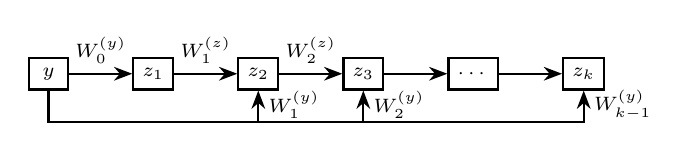
\begin{tikzpicture}[
        >={Stealth},
        thick,
        node distance=0.8cm and 0.8cm,
        every node/.style={draw, rectangle, minimum height=0.4cm, minimum width=0.5cm, font=\scriptsize},
        every path/.style={->}
      ]

      % Nodes
      \node (y) {$y$};
      \node[right=of y] (z1) {$z_1$};
      \node[right=of z1] (z2) {$z_2$};
      \node[right=of z2] (z3) {$z_3$};
      \node[right=of z3] (dots) {$\cdots$};
      \node[right=of dots] (zk) {$z_k$};

      % Connections
      \draw[->] (y) -- (z1) node[midway, above, draw=none] {$W_0^{(y)}$};
      \draw[->] (z1) -- (z2) node[midway, above, draw=none] {$W_1^{(z)}$};
      \draw[->] (z2) -- (z3) node[midway, above, draw=none] {$W_2^{(z)}$};
      \draw[->] (z3) -- (dots);
      \draw[->] (dots) -- (zk);

      % Vertical Loops
      \draw[->] (y) |- ([yshift=-0.4cm] z2.south) -- (z2.south) node[pos=0.55, right, draw=none] {$W_1^{(y)}$};
      \draw[->] (y) |- ([yshift=-0.4cm] z3.south) -- (z3.south) node[pos=0.55, right, draw=none] {$W_2^{(y)}$};
      \draw[->] (y) |- ([yshift=-0.4cm] zk.south) -- (zk.south) node[pos=0.55, right, draw=none] {$W_{k-1}^{(y)}$};

    \end{tikzpicture}
    \caption{Input Convex Neural Network (ICNN) Structure.}
    \label{f3}
\end{figure}

\citet{Amos17} introduced Input Convex Neural Networks (ICNNs) to model convex functions by optimizing a set of parameters, \(\{W_{i}^{(y)}, W_{i}^{(z)}\}\), during each iteration.

Given an initial input \(y\), the ICNN learns the convex function \(z_k\) through the following formulation:
\[
z_{i+1} = g_i \left( W_i^{(z)} z_i + W_i^{(y)} y + b_i \right), \quad f(y; \theta) = z_k,
\]
where \(z_i\) represents the layer activations, \(\theta = \left\{ W_{0:k-1}^{(y)}, W_{1:k-1}^{(z)}, b_{0:k-1} \right\}\) denotes the model parameters (\(W_{0:k-1}^{(y)}\) and \(W_{1:k-1}^{(z)}\) are weight matrices, and \(b_{0:k-1}\) are bias terms), and \(g_i\) is a non-linear activation function. During each iteration, a small batch is drawn from both the source and target domains, and the ICNN learns \(f\) and \(g\) within \(\mathtt{ICNN}(\mathbb{R}^d)\) by optimizing the minimax problem with parameters \(\theta_f\) and \(\theta_g\).

To ensure the convexity of the network, weights $W_{i}^{(y)}$ and $W_{i}^{(z)}$ must remain non-negative. \citet{Makkuva20} demonstrated the feasibility of adding an arbitrary bounds to \(\theta\) during the training process; This implementation indicates that \(\theta_f\) and \(\theta_g\) can be learned from a compact and uniformly bounded function space $\mathtt{ICNN}(\mathbb{R}^d)$ given $P,Q\in \mathbb{R}^d$, which could simplify the original convex function space by restricting it to a smaller subspace compatible with $\mathtt{ICNN}(\mathbb{R}^d)$:
\begin{assumption}\label{a3.1}
We assume that both source measure $P$ and target measure \(Q\) admits a density with respect to the Lebesgue measure, and that there exist convex subsets \(\mathcal{S}(P) \subset \mathtt{CVX}(P)\) and \(\mathcal{S}(Q) \subset \mathtt{CVX}(Q)\) which are uniformly bounded. During the ICNN training, we have \(
\mathtt{ICNN}(\mathbb{R}^d) \subset \mathcal{S}(P) \) and \(
\mathtt{ICNN}(\mathbb{R}^d) \subset \mathcal{S}(Q).\)
\end{assumption}
\begin{proposition}
\label{p3.2}
Under Assumption~\ref{a3.1}, there exists an optimal solution \((f_0, g_0)\). Furthermore, the corresponding optimal transport map \(T\) from \(Q\) to \(P\) can be directly recovered via \(\nabla g_0\).
\end{proposition}

\subsection{Sparsity-inducing Penalties $\tau$}
\label{sec3.3}
\citet{Cuturi23} proposed the following cost function to induce displacement sparsity:
\[
c(\mathbf{x}, \mathbf{y}) = \frac{1}{2} \| \mathbf{x} - \mathbf{y} \|_{2}^2 + \lambda \cdot \tau(\mathbf{y} - \mathbf{x}). \tag{5} \label{e5}
\]
Under this regularized cost, the optimal transport mapping can be expressed as:
\[
T(\mathbf{x}) = \mathbf{x} - \mathrm{prox}_{\tau} \left( \mathbf{x} - \sum_{j=1}^m p^j(\mathbf{x}) \left( \mathbf{y}^j + \nabla\tau(\mathbf{x} - \mathbf{y}^j) \right) \right),
\]
where $\mathrm{prox}_{\tau}$ denotes the proximal operator of $\tau$, and $p^j(\mathbf{x})$ represents the $\mathbf{x}$-dependent Gibbs distribution over the $m$-simplex. \citet{Cuturi23} introduced three choices for the penalty function $\tau$: the $\ell_{1}$-norm, Vanishing Shrinkage STVS ($\tau_{\text{stvs}}$), and $k$-overlap norm \cite{NIPS2012_99bcfcd7}. However, the $k$-overlap was ultimately abandoned due to its undesirable computational cost.

\textbf{\(\ell_{1}\)-Norm.} The \(\ell_{1}\)-norm directly penalizes the magnitude of the displacement vector, encouraging it to move towards the nearest target and inducing sparsity.

\textbf{Vanishing Shrinkage STVS.} \citet{schreck2015shrinkage} introduce the soft-thresholding operator with vanishing shrinkage (STVS) for displacement vector $\mathbf{z}$,
\[
\tau_{\text{stvs}}(\mathbf{z}) = \gamma^2 \mathbf{1}_d^T \left( \sigma(\mathbf{z}) + \frac{1}{2} - \frac{1}{2} e^{-2 \sigma(\mathbf{z})} \right), 
\]
where \(\sigma(\mathbf{z})=\operatorname{asinh}(\frac{z}{2\gamma})\) with element-wise operations.

However, both the $\ell_1$-norm and $\tau_{\text{stvs}}$ fail to directly reflect the dimensionality of the displacement vector. To address this, we introduce the most straightforward dimensionality penalty, the $\ell_{0}$-norm, into our model. Empirically, we find that a smoothed version of the $\ell_{0}$-norm is more suitable for the gradient descent scheme in ICNN training.

\textbf{Smoothed $\ell_{0}$-Norm.} To approximate the discontinuous $\ell_{0}$-norm, \citet{10.1007/978-3-540-74494-8_49} proposed replacing the indicator function \(\nu(\mathbf{z})\), where \(\nu(\mathbf{z}) = 1\) if \(\mathbf{z} \neq 0\) and \(\nu(\mathbf{z}) = 0\) otherwise, with a smooth Gaussian function:
\[
f_{\sigma}(\mathbf{z}) = \exp\left(-\frac{\mathbf{z}^2}{2\sigma^2}\right).
\]
As \(\sigma \to 0\), \(f_{\sigma}(\mathbf{z})\) approximates \(1 - \nu(\mathbf{z})\). The smoothed \(\ell_{0}\)-norm is thus given by $n - \displaystyle\sum_{i=1}^n f_{\sigma}(\mathbf{z}_i)$.
Note that the smoothed \(\ell_{0}\)-norm is non-convex, meaning its proximal operator may not be well defined and therefore cannot be directly applied to (\hyperref[e5]{5}) to recover the mapping \(T\).

\section{Sparsity-inducing Minimax Formulation}\label{s4}
Our goal is to bring sparsity to the displacement vector  \(\Delta(\mathbf{x}):= T(\mathbf{x}) - \mathbf{x}\) from the map $T$ learned via ICNN, making the result with better interpretability. We introduce the sparsity penalty to the minimax formulation (\hyperref[e4]{4}), which makes the squared 2-Wasserstein biased:
\begin{align}
\widetilde{W_2^2}(P, Q) = C_{P,Q} + &\sup_{f \in \mathcal{S}(P)} \inf_{g \in \mathcal{S}(Q)} \mathcal{V}_{P,Q}(f, g) \notag \\
&\quad + \lambda \int_{\mathbb{R}^d} \tau \left( \nabla g(y) - y \right) \, dQ, \tag{6} \label{e6}
\end{align}
where \(\nabla g(y) - y\) represents displacement vector derived from (\hyperref[e4]{4}), and \(\lambda\) is a parameter that controls the intensity of sparsity-inducing.

As discussed in §\hyperref[sec3.1]{3.1}, it is infeasible to re-parameterize the dual potentials into (\hyperref[e4]{4}) when the quadratic cost is not used. Therefore, we adopt an intuitive approach to penalize the map as a whole. In this formulation, any $\tau$ function can be applied to recover the mapping without relying on $\mathrm{prox}_{\tau}$. Leveraging ICNN, we propose a heuristic framework in §\hyperref[sec4.1]{4.1} that dynamically adjusts the intensity $\lambda$ based on different goals, a feature not applicable to traditional Sinkhorn solvers. Several theoretical guarantees are introduced:
\begin{lemma} \label{l4.1}
Let $\tau$ be the sparsity penalty introduced in \S\hyperref[sec3.3]{3.3}. Assume that $P$ and $Q$ are probability measures over $\mathbb{R}^d$ with bounded support. Moreover, suppose that $\mathcal{S}(P)$ and $\mathcal{S}(Q)$ contains only L-Lipschitz continuous functions $f$ and \( g \) respectively. Then, the sparsity penalty \(\int_{\mathbb{R}^d} \tau \left( \nabla g(y) - y \right) \, dQ\) is bounded for any \( g \in \mathcal{S}(Q) \).
\end{lemma}

\textbf{Remark 4.1.} The bounded support assumption for $Q$ in Lemma \hyperref[l4.1]{4.1} is reasonable, as it is feasible to impose arbitrary bounds on the parameters within the $\mathtt{ICNN}(\mathbb{R}^d)$ training space, proposed by \citet[Remark 3.4]{Makkuva20}. This assumption holds for the rest theoretical results in \S\hyperref[s4]{4}.

\begin{theorem}\label{t4.3}Let \( J_{0} \) denote the Wasserstein distance as defined in equation (\hyperref[e4]{4}), and let \( J_{\lambda} \) denote the biased Wasserstein distance as defined in equation (\hyperref[e6]{6}). Then, we have:
\[
\lim_{\lambda \to 0} J_{\lambda} = J_{0}.
\]
\end{theorem}
\begin{theorem}\label{t4.4}Let \(\mathcal{G}\subseteq \mathcal{S}(Q)\times \mathcal{S}(P)\) be the closed set of optimal solutions 
\(\bigl(g_{0}, f_{0}\bigr)\) to the optimization problem in 
\eqref{e4}, and let \(\bigl(g_{\lambda}, f_{\lambda}\bigr)\) be an optimal solution of \eqref{e6}, 
for a given \(\lambda \ge 0\) and a convex regularizer \(\tau\), we have
\[
\lim_{\lambda \to 0} 
\mathrm{dist}\Bigl(\bigl(g_{\lambda}, f_{\lambda}\bigr),\, \mathcal{G}\Bigr) 
\;=\; 0,
\]
where
\(\mathrm{dist}\bigl((g,f), \mathcal{G}\bigr) \;=\; 
\inf_{(g_0,f_0)\in \mathcal{G}} 
\bigl\|\,(g,f)-(g_0,f_0)\,\bigr\|\)
denotes the distance from the point \(\bigl(g,f\bigr)\) to the set \(\mathcal{G}\) 
in an appropriate normed space.
\end{theorem}
Note that \((g_{\lambda}, f_{\lambda})\) converges to a unique \((g_{0}, f_{0})\) only if the objective function is strongly concave-strongly convex.
\begin{theorem}\label{t4.5} Let \((g_{\lambda_{1}}, f_{\lambda_{1}})\) and \((g_{\lambda_{2}}, f_{\lambda_{2}})\) be the optimal solutions to the optimization problem defined in equation (\hyperref[e6]{6}) for \(\lambda = \lambda_{1}\) and \(\lambda = \lambda_{2}\), respectively, where \(0 \leq \lambda_{1} < \lambda_{2}\), and let \(\tau\) be a convex regulator. Then, the following inequality holds:
\[
\int_{\mathbb{R}^d} \tau (\nabla g_{\lambda_{1}}(y) - y) \, dQ \geq \int_{\mathbb{R}^d} \tau (\nabla g_{\lambda_{2}}(y) - y)\, dQ.
\] 
\end{theorem}

Theorem \hyperref[t4.3]{4.2} establishes that the formulation remains unbiased in the limit as \(\lambda \to 0\). Theorem \hyperref[t4.4]{4.3} demonstrates the convergence of the dual potentials specifically for convex regulators. Theorem \hyperref[t4.5]{4.4} shows the monotonicity of the map's sparsity level as \(\lambda\) increases. However, we empirically observe that our non-convex regulators also exhibit these properties, as discussed in a later section. Proofs of these theorems and Lemma \hyperref[l4.1]{4.1} are provided in Appendix \hyperref[A1]{A}. The proofs proceed by first establishing Lemma \hyperref[lA2]{A.2}, which, combined with \citet{vonNeumann1928}'s Minimax Theorem, are used to prove the rest of the theorems. Examples of mappings learned with different $\tau$ penalties and a constant $\lambda$ are shown in Figure \hyperref[f1]{1}.

To align with ICNN training, we restrict our training space in (\hyperref[e6]{6}) from $\mathcal{S}(P)$ and $\mathcal{S}(Q)$ to its subspace $\mathtt{ICNN}(\mathbb{R}^d)$:
\begin{align}
\widetilde{W_2^2}(P, Q) = C_{P,Q} + &\sup_{f \in \mathtt{ICNN}(\mathbb{R}^d)} \inf_{g \in \mathtt{ICNN}(\mathbb{R}^d)} \mathcal{V}_{P,Q}(f, g) \notag \\
&\quad + \lambda \int_{\mathbb{R}^d} \tau \left( \nabla g(y) - y \right) \, dQ, \tag{7} \label{e89}
\end{align}

We also establish a bound on the deviation of the optimal transport map \(\nabla g_{\lambda}\) in (\hyperref[e6]{6}). For brevity, define  
\[
\mathcal{N}_{P,Q}(f,g) = \mathcal{V}_{P,Q}(f,g) + \lambda \int_{\mathbb{R}^d} \tau(\nabla g(y) - y) \, dQ,
\]
 Let \((g_{\lambda}, f_{\lambda})\) denote the optimal solution to the minimax problem \((\hyperref[e6]{6})\). For any pair \((g, f)\), the minimization gap \(\epsilon_1\) and maximization gap \(\epsilon_2\) are defined as follows:
\[
\epsilon_1(f, g) = \mathcal{N}_{P,Q}(f, g) - \inf_{g' \in \mathcal{S}(Q)} \mathcal{N}_{P,Q}(f, g') \geq 0,
\]
\[
\epsilon_2(f) = \mathcal{N}_{P,Q}(f_{\lambda}, g_{\lambda}) - \inf_{g' \in \mathcal{S}(Q)} \mathcal{N}_{P,Q}(f, g') \geq 0.
\]
From Lemma \hyperref[l4.1]{4.1}, the penalty term \(\tau(\nabla g(y) - y)\) is bounded. For simplicity, let
\(s(g) = \int_{\mathbb{R}^d} \tau(\nabla g(y) - y) \, dQ,\)
where \(s(g)\) is bounded between 0 and \(M_{\tau}\), with \(M_{\tau}\) being a constant depending on \(\tau\) (details provided in Appendix \hyperref[A1]{A}). Consequently, the sparsity gap between any two functions \(g_i\) and \(g_j\), given by \(\|s(g_i) - s(g_j)\|\), is also bounded by \(M_{\tau}\). With the definitions of \(\epsilon_1\), \(\epsilon_2\), and \(M_{\tau}\), we can derive a bound on the deviation of the optimal transportation map.

\begin{theorem}\label{t4.6}
Consider \(\nabla g_{0}\) to be the unbiased ground truth map from \(Q\) to \(P\) under formulation (\hyperref[e4]{4}). For $\lambda >0$ and any other pair \((g, f)\), where \(f\) is \(\alpha\)-strongly convex, the following bound holds for solving biased map from formulation (\hyperref[e6]{6}):
\[
\|\nabla g - \nabla g_{0}\|^2_{L^2(Q)} \leq \frac{2}{\alpha} \left( \epsilon_1 + \epsilon_2 + 2\lambda M_{\tau} \right).
\]
\end{theorem}
Larger $\lambda$ would therefore cause the actual-solved map diverging more to the theoretical optimized map. The proof is provided in Appendix \hyperref[A1]{A}. It builds upon the unbiased formulation bound established by \citet{Makkuva20}, with additional consideration for the sparsity gap.

\subsection{Dynamic Adjustment to Sparsity Intensity $\lambda$} \label{sec4.1}
\begin{figure*}[ht!]
    \centering
    \begin{minipage}[t]{0.62\textwidth} 
        \centering
        \includegraphics[width=0.75\textwidth]{A.pdf} 
    \end{minipage}%
    \hfill
    \begin{minipage}[t]{0.38\textwidth}
        \centering
        \includegraphics[width=\textwidth]{C.pdf} 
    \end{minipage}
    \vspace{-2em}
    \caption{\textbf{Left}: Two classic eight-Gaussian examples are presented, where the source measure is located at the center, and eight target measures are generated from Gaussian distributions. These examples illustrate the trade-off between the sparsity of the map and its feasibility under varying values of $\alpha$. \textbf{Right}: A simulation example demonstrates how $\lambda$ changes during simulated annealing training under $\alpha=0.9$, along with the corresponding levels of map sparsity (Spa) and feasibility (Res).}
    \label{f4}
\end{figure*}
In the previous section, we utilized a constant \(\lambda\) to enforce sparsity in the learned map via ICNN. However, this approach presents inherent challenges: if \(\lambda\) is set too low, the resulting map lacks sufficient sparsity, failing to promote the desired regularization. Conversely, if \(\lambda\) is set too high, the accuracy of the map degrades, leading to a larger deviation of \(T_{\#}(P)\) from the true target \(Q\). This trade-off is clearly illustrated in Figure~\hyperref[f2]{2} and additional example Figure~\hyperref[f4]{4}, where we use the classic eight-Gaussian setup to demonstrate this effect. Note that eight-Gaussian example is intended solely for illustrative purposes, as sparsity is not a necessary requirement in this context. In the extreme sparsity case, more and more points collapse towards the source center without adequate transportation to their targets.

We introduce a parameter $\alpha$ to tune this tradeoff by dynamically adjusting \(\lambda\) to optimize a goal function that balances sparsity and feasibility during the ICNN training process. For the map \(T_{n}: X\rightarrow Y\) learned at the \(n\)-th iteration of ICNN training, we define its sparsity and feasibility level through two metrics, Spa (Sparsity) and Err (Error), where
\[\text{Spa} = \int_P \tau(T_n(x) - x) \, dP, \quad \text{Err}=D(T_{n\#}(P), Y).\]
We use the corresponding sparsity metric, $\tau$, during training, while measuring the error through the divergence $D$ between the mapped distribution and the actual target distribution. To capture this geometric divergence, we approximate the source and target distributions, $P$ and $Q$, as finite sets of sampled points, and use the Wasserstein distance to quantify the divergence between them. However, due to the computational inefficiency of the Wasserstein distance, we accelerate the training process by approximating it with the sliced Wasserstein distance \cite{bonneel2015sliced}. 

It is important to normalize both metrics to the same numerical scale. Ultimately, we construct the evaluation function:
\[
\label{e7}
\text{Eval} = \alpha \cdot \text{Spa} + (1 - \alpha) \cdot \text{Err}, \quad \alpha \in [0,1], \tag{8}
\]
where \(\alpha\) is a pre-determined parameter. A higher value of \(\alpha\) leads to a higher sparsity-inducing intensity. The objective is to find the \(\lambda\) that minimizes \(\text{Eval}\). Since \(\lambda\) is not explicitly related to \(\text{Eval}\), we use the heuristic search by embedding a simulated annealing framework into ICNN, leveraging from its ability to swiftly adapt to adjustments in \(\lambda\). We heuristically adjust \(\lambda\) after every specific number of iterations (to give the ICNN sufficient time to smoothly adjust the map with the updated \(\lambda\)). Example of simulation are illustrated in Figure~\hyperref[f4]{4}, and the algorithm pipeline is shown in Algorithm \hyperref[al1]{1}.

\begin{algorithm}[h]
\caption{Heuristic Adjustment Framework for $\lambda$}
\label{al1}
\textbf{Input:} $\alpha$, $\lambda$, $n_{\text{ini}}$, $n_{\text{tr}}$ $n_{\text{sm}}$; Initial temperature $Tem$, Min temperature $Tem_{\min}$, Decay rate $d$
\begin{algorithmic}[1]
\STATE \textbf{Initialize:} Train dual potentials $f, g$ with $\lambda$ for $n_{\text{ini}}$ iterations until stable.

\WHILE{$Tem > Tem_{\min}$}
    \STATE $\lambda \gets \text{SimulatedAnnealing}(Tem, \lambda)$
    \STATE map $T_{n} \gets$ Train $f, g$ with updated $\lambda$ for $n_{\text{tr}}$ iterations
    \STATE $\text{Eval}_{n} \gets \text{Eval}(T_{n})$
    \STATE Accept or reject $\lambda$ based on $\text{Eval}_{n}$
    \IF{Rejected}
        \STATE Smoothly revert using $n_{\text{sm}}$ iterations of training.
    \ENDIF
    \STATE $Tem \gets Tem \cdot d$.
\ENDWHILE
\end{algorithmic}
\end{algorithm}

In the simulated annealing framework, we first perform \(n_{\text{ini}}\) iterations using the starting value of \(\lambda\) to train dual potentials until the map's sparsity and error levels converge to a stable state. After reaching this initial stability, we initiate the simulated annealing process with a starting temperature \(T\). We then continue training duel potentials with the new \(\lambda\) for \(n_{\text{tr}}\) iterations. To ensure smooth transitioning, if the new \(\lambda\) is not accepted, we perform an additional \(n_{\text{sm}}\) iterations of training to allow the ICNN to revert smoothly to the previous value of \(\lambda\).

\subsection{High Dimensional Setting} 
\label{sec4.2}
In the high-dimensional setting, a separate framework is required, as it is impractical to impose a sparsity constraint directly on the low dimensional displacement vectors. Instead of using the metric to evaluate the map sparsity level, we adopt a more feasible approach by constraining the dimensionality of the displacement vectors in the high-dimensional space. Specifically, given \( P, Q \in \mathbb{R}^d \), our goal is to find an optimal transport map \( T \) such that all displacement vectors \( \Delta(\mathbf{x}) = T(\mathbf{x}) - \mathbf{x} \) lie within a subspace of dimensionality less than \( l \), where \( l < d \). Among all maps that satisfy this dimensionality constraint, we aim to find the one that minimizes the divergence between \( T_{\#}(P) \) and \( Q \). This optimization problem can be formulated as follows:
\[
\begin{aligned}
    \min_{T} \quad & \frac{1}{2} \mathbb{E}_{X \sim P} \left\|T(X) - X\right\|^2 + \beta D(T_{\#}(P), Q) \\
    \text{s.t.} \quad & \dim(T(x_i) - x_i) \leq l, \quad l < d, \quad \forall x_i \in X.
\end{aligned}
\label{e8}
\]
By introducing a divergence regularization term \(D(T_{\#}(P), Q)\) with weighting parameter \(\beta\), we relax the requirement that the source measure \(P\) must be exactly transported to the target measure \(Q\) (i.e., \(T_{\#}(P) = Q\)). This formulation is indeed challenging to solve with traditional methods due to the direct constraint on the dimensionality of the vectors. However, our new heuristic framework based on ICNN can efficiently address this problem by doing minor adaptions to Algorithm \hyperref[al1]{1}. 

Specifically, we can directly apply the smoothed \(\ell_{0}\)-norm to regularize the dimensionality of the displacement vectors. Although the smoothed \(\ell_{0}\)-norm is not a convex penalty, we empirically observe that increasing \(\lambda\) enhances sparsity, as shown in Figure \hyperref[f5]{5}. Therefore, our strategy to adjust \(\lambda\) becomes straightforward: we initially increase \(\lambda\) until the dimensionality requirement is met; then, we decrease \(\lambda\) to minimize \(D(T_{\#}(P), Q)\) while maintaining the dimensionality constraint. All the adjustments towards $\lambda$ are still working on a heuristic framework in Algorithm \hyperref[al1]{1}. Detailed pipeline can be found in Appendix \hyperref[aphh]{B}.

\section{Experiments}
\textbf{Drug Perturbation \& Optimal Transport.} Optimal transport has become a powerful tool in cell biology for modeling and predicting cellular responses to drug perturbations \cite{Bunne23}. It matches perturbed cells to their original state by measuring high-dimensional features such as single-cell RNA (sc-RNA) expression and 4i (Iterative Indirect Immunofluorescence Imaging) data.

We conducted experiments to evaluate the performance of our sparsity-induced formulation against the original ICNN OT framework and compared it to the Sinkhorn-based sparsity formulation proposed by \citet{Cuturi23} on two different cell matching tasks.
\begin{figure}[H]
    \centering
    \includegraphics[width=0.8\columnwidth,height=0.14\textheight]{Fig4.pdf} 
    \vspace{-1em} 
    \caption{Synthesized sc-RNA perturbation dataset with \( n=4000 \) cells, \( d=3000 \) genes, and \( k=100 \) genes. An OT mapping was learned between the control and treated cells. The average displacement dimensionality during training iterations is shown.}
    \label{f5}
\end{figure}

\subsection{Synthesized sc-RNA Perturbation Task} \label{sec5.1}
Because our first aim was to measure how closely our method could reduce dimensionality to the ground-truth level, we did not run the first task on a real sc-RNA dataset. As real sc-RNA data is unable to allow a reliably accurate determination of the ground truth displacement dimensionality, we built a synthesized dataset for this task, leaving the real dataset for subsequent experiments.

The dataset is constructed as follows: we first define \( n \), the number of cells before and after drug perturbation; \( d \), the total number of genes per cell (overall dimensionality); and \( k \), the number of genes truly affected by the drug (ground-truth dimensionality). Random noise is added to the remaining genes to simulate realistic noise observed in drug perturbation scenarios. The control cells are treated as the source, and the perturbed cells are treated as the target. Using different methods, we compute the OT mapping between two groups of cells. Our objective is to evaluate whether these methods can provide an explainable mapping that focuses exclusively on the truly perturbed genes while disregarding the noisy ones. Example result is shown in Figure \hyperref[f5]{5}.

We compare three different methods: ICNN OT, \citet{Cuturi23}'s approach with the \(\ell_1\)-norm penalty, and our formulation with the smoothed \(\ell_0\)-norm penalty under different sparsity-intensity levels (\(\lambda\)). Results in Figure \hyperref[f5]{5} show that, comparing to ICNN OT, our formulation effectively reduces the dimensionality of the displacement map towards the ground-truth level. \citet{Cuturi23}'s method produces results closest to the ground-truth map. However, neural OT solvers are often preferred in real drug perturbation scenarios because they efficiently handle large, high-dimensional single-cell data, incorporate domain-specific constraints, and are flexible to varying inputs. In contrast, traditional Sinkhorn solvers require storing large cost matrices and multiple iterative updates, making them less scalable.
\begin{table}[h]
\centering
\vspace{-1.5em}
\caption{Comparison of different methods' performance.}
\label{tab:ot_comparison}
\resizebox{0.5\textwidth}{!}{%
\begin{tabular}{lccccc}
\toprule
\textbf{Method}        & \multicolumn{1}{c}{\textbf{ICNN OT}} & \multicolumn{1}{c}{\textbf{Cuturi et al. (2023)}} & \multicolumn{3}{c}{\textbf{Our Formulation}} \\ 
\cmidrule(lr){2-2} \cmidrule(lr){3-3} \cmidrule(lr){4-6}
                       &                                      &                                                   & $\lambda = 5 \times 10^{-4}$ & $\lambda = 1 \times 10^{-3}$ & $\lambda = 5 \times 10^{-3}$ \\
\midrule
\textbf{dim($\Delta(\mathbf{x})$)}         & 2480                                 & 99                                                & 153                          & 138                          & 120                          \\
\bottomrule
\end{tabular}%
}
\end{table}
\vspace{-1.5em}
\begin{figure*}[ht!]
    \centering
    \includegraphics[width=0.88\textwidth]{Figure6.pdf}
    \vspace{-1.2em}
    \caption{The results of the 4i ($d=78$ features) perturbation under four different drugs are presented. Each experiment, conducted at a specific $\lambda$, displays the average outcome of ten runs. $\lambda^{(i)}$ represents the ordered statistics of each set of $\lambda$ used in the experiments. Due to the inherent differences in the drugs, $\lambda^{(i)}$ varies across the experiments. \texttt{np.isclose(.,0)} is evaluated at the threshold of $10^{-2}$ to determine the dimensionality of the displacement vectors. Number of cells, $n$, in each experiment is approximately $12,000$ cells.}
    \label{f6}
\end{figure*}
\subsection{Real 4i Perturbation Task} \label{sec5.2}
In this section, we use the preprocessed cell 4i perturbation dataset\footnote{Dataset is publicly available at the following \href{https://www.research-collection.ethz.ch/handle/20.500.11850/609681}{site} \cite{20.500.11850/609681}.}, designed for optimal transport matching as utilized in CellOT \cite{Bunne23}, to demonstrate the effect of sparsity induction on the displacement vector.

This task assesses the effectiveness of various methods in recovering the OT map, focusing on preserving key features while disregarding less significant ones. Unlike sc-RNA perturbation, where there is a clear separation between noisy and genuinely perturbed cells, recovering the OT map is notably more challenging. Additionally, the absence of a ground-truth map with the true dimensionality further complicates the task. After drug perturbation, the 4i features of the cells are altered, and we use these features to match control cells with perturbed cells. To evaluate the learned map $T$, we employ two metrics: (\textbf{i}) Average displacement vector dimensionality – \textit{lower values indicate better interpretability}; (\textbf{ii}) Wasserstein divergence between $T_{\#}(P)$ and $Q$ – \textit{lower values indicate better feasibility}.

We selected four drugs (Ixazomib, Sorafenib, Cisplatin, Melphalan) to highlight the improvement of our method towards the existing methods. As shown in Figure \hyperref[f6]{6}, among all four drugs, our method could more effectively reduce the dimensionality of the displacement vector. However, several limitations need to be discussed here:

\textbf{Variance of the Results.} Due to the inherent randomness in ICNN, the results typically exhibit higher instability as $\lambda$ increases, leading to more varied outcomes across runs. This aligns with Theorem \hyperref[t4.6]{4.5}, which gives that a larger $\lambda$ results in a higher error bound. In contrast, the Sinkhorn-based method introduced by \citet{Cuturi23} consistently achieves convergence in its learned mappings.

\textbf{Unknown and Varied Minimized Dimensionality.} The minimized dimensionality in each experiment varies and is data-driven, making it difficult and impractical to estimate a theoretical or empirical minimum. Therefore, for some dimensionality constraint $l$ from the constrained optimization in \S\hyperref[sec4.2]{4.2}, it may result in no solutions.

\textbf{Non-convex Penalty under Theoretical Guarantee.} Our theoretical guarantee (Theorem \hyperref[t4.4]{4.3}, \hyperref[t4.5]{4.4}) only applies to convex penalties. However, the smoothed \(\ell_{0}\)-norm is pseudoconvex and therefore does not benefit from the theoretical guarantee. This can be observed in the dimensionality for the highest $\lambda$ in each experiment, where the average dimensionality begins to increase. Non-convexity might be a contributing factor, but it is worth noting that the metric used to measure sparsity in Theorem \hyperref[t4.5]{4.4} is the penalty function $\tau$, whereas we use the direct dimensionality metric in the experiment. All the hyper-parameters setup for each experiments in this work are detailed in Appendix \hyperref[hyp]{C}.
\section{Conclusions}
We presented a biased, sparsity-inducing formulation based on the unbiased formulation from ICNN OT and demonstrated its reliability in recovering maps with higher displacement sparsity in both low- and high-dimensional experiments. Leveraging ICNN, we also provide a heuristic framework with a flexible objective that can dynamically adjust the sparsity-inducing intensity. Additionally, we adapt this framework to solve the problem with direct constraint on displacement dimensionality in higher-dimensional setting. Several future directions could stem from our work, encompassing both theoretical and empirical aspects. On the theoretical side, these include estimating the theoretical minimized dimension and applying the sparsity-inducing framework to other neural OT solvers (e.g., non-minimax formulations). On the empirical side, directions include studying the effects of hyperparameters and fine-tuning those used in our heuristic framework.
\section*{Impact Statement}
This paper presents work whose goal is to advance the field of Machine Learning. There are many potential societal consequences of our work, none which we feel must be specifically highlighted here.

\section*{Acknowledgement}
PC is partially supported by the HKU-IDS Research Grant. YX is supported by Guangdong Province Fundamental and Applied Fundamental Research Regional Joint Fund, (Project 2022B1515130009), and the start-up fund of HKU-IDS.  QZ is supported by the National Natural Science Foundation of China (grant no. 71972164) and the Research Grant Council of Hong Kong SAR Government (grant no. 11218221).

This work is supported by computing resources from the HKU-Shanghai ICRC cluster. We would also like to thank Fei Jing from QZ's group for his assistance.
\bibliography{example_paper}
\bibliographystyle{icml2024}

%%%%%%%%%%%%%%%%%%%%%%%%%%%%%%%%%%%%%%%%%%%%%%%%%%%%%%%%%%%%%%%%%%%%%%%%%%%%%%%
%%%%%%%%%%%%%%%%%%%%%%%%%%%%%%%%%%%%%%%%%%%%%%%%%%%%%%%%%%%%%%%%%%%%%%%%%%%%%%%
\newpage
\appendix
\onecolumn
\section{Proofs of Theorems}
\label{A1}

\noindent \textbf{Proof of Lemma \hyperref[l4.1]{4.1}:} Given the assumption on the bounded support of the target measure and the boundedness of $\nabla g$, which is implied by the uniform \emph{Lipschitiz} continuity of $g$ in $\mathcal{S}(Q)$ and convexity, we can to show that \(\tau(\cdot)\) is bounded:
\begin{itemize}
  \item The smoothed \(\ell_{0}\)-norm is bounded because the dimensionality of the target measures is bounded.
  \item The \(\ell_{1}\)-norm is bounded because the magnitude of the displacement vectors is bounded.
  \item By the Weierstrass theorem, \(\tau_{\mathrm{stvs}}\) is bounded on the compact region covering the value of $\nabla g(y)-y$ since it is continuous.
\end{itemize}
Given these bounds, we can conclude that Lemma  \hyperref[l4.1]{4.1} holds for all three sparsity penalties used in our analysis.

\begin{theorem}[von Neumann's Minimax Theorem] \label{minimax}
Let \( X \subset \mathbb{R}^n \) and \( Y \subset \mathbb{R}^m \) be two compact and convex sets. Suppose \( f: X \times Y \to \mathbb{R} \) is a continuous function that is concave in \( x \) for each fixed \( y \) and convex in \( y \) for each fixed \( x \) (concave-convex). Then, the following equality holds:
\[
\max_{x \in X} \min_{y \in Y} f(x, y) = \min_{y \in Y} \max_{x \in X} f(x, y).
\]
\noindent Moreover, assuming the optimal solution $(x^*, y^*)$ exists, then it satisfies the following saddle point inequality:
\[
f(x,y^*)\leq f(x^*, y^*) \leq f(x^*, y),\quad \forall x \in X, y \in Y,\
\]
\end{theorem}
In the context of ICNN, our sets $X$ and $Y$ are instead topological vector spaces, which places them under the scope of a variant of von Neumann’s Minimax Theorem: Sion’s Minimax Theorem \cite{sion}.
\begin{lemma}\label{lA2}
For equation (\hyperref[e4]{4}), given \( f \in \mathtt{CVX}(P) \) and \( g \in \mathtt{CVX}(Q) \), the function
\[
\mathcal{V}_{P,Q}(f, g) = -\mathbb{E}_P[f(X)] - \mathbb{E}_Q\left[\langle Y, \nabla g(Y)\rangle - f(\nabla g(Y))\right]
\]
is a concave-convex and continuous function.
\end{lemma}

\noindent \textbf{Proof of Lemma A.2 --- \emph{Concave-Convex}:} To prove that \( \mathcal{V}_{P,Q}(f, g) \) is a concave-convex function, we first show that, for a fixed \( g \), \( \mathcal{V}_{P,Q}(f, g) \) is concave in \( f \).

Consider any two functions \( f_{1}, f_{2} \in \mathtt{CVX}(P) \) and any \( \alpha \in [0,1] \). We aim to show that:
\[
\mathcal{V}_{P,Q}(\alpha f_{1} + (1-\alpha) f_{2}, g) \geq \alpha \mathcal{V}_{P,Q}(f_{1}, g) + (1-\alpha) \mathcal{V}_{P,Q}(f_{2}, g). \tag{9} \label{e9}
\]
To demonstrate this, note that by linearity:
\begin{align*}
\mathcal{V}_{P,Q}(\alpha f_{1} + (1-\alpha) f_{2}, g) &= -\mathbb{E}_P[(\alpha f_{1} + (1-\alpha) f_{2})(X)] \\
&\quad - \mathbb{E}_Q\left[\langle Y, \nabla g(Y)\rangle - (\alpha f_{1} + (1-\alpha) f_{2})(\nabla g(Y))\right] \\
&= - \alpha \mathbb{E}_P[f_{1}(X)] - (1-\alpha) \mathbb{E}_P[f_{2}(X)] \\
&\quad + \alpha \mathbb{E}_Q\left[f_{1}(\nabla g(Y))\right] + (1-\alpha) \mathbb{E}_Q\left[f_{2}(\nabla g(Y))\right] \\
&\quad - \mathbb{E}_Q\left[\langle Y, \nabla g(Y)\rangle\right] \\
&= \alpha \mathcal{V}_{P,Q}(f_{1}, g) + (1-\alpha)\mathcal{V}_{P,Q}(f_{2}, g).
\end{align*}
This establishes that \( \mathcal{V}_{P,Q}(f, g) \) is concave in \( f \) for a fixed \( g \).

Next, we show that for a fixed \( f \), \( \mathcal{V}_{P,Q}(f, g) \) is convex in \( g \). Consider any \( g_{1}, g_{2} \in \mathtt{CVX}(Q) \) and any \( \alpha \in [0,1] \). We need to prove that:
\[
\mathcal{V}_{P,Q}(f, \alpha g_{1} + (1-\alpha) g_{2}) \leq \alpha \mathcal{V}_{P,Q}(f, g_{1}) + (1-\alpha)\mathcal{V}_{P,Q}(f, g_{2}). \tag{10} \label{e10}
\]
By definition, we have:
\begin{align*}
\mathcal{V}_{P,Q}(f, \alpha g_{1} + (1-\alpha) g_{2}) 
&= -\mathbb{E}_P[f(X)] \\
&\quad - \mathbb{E}_Q\left[\langle Y, \alpha \nabla g_{1} (Y) + (1-\alpha) \nabla g_{2}(Y)\rangle - f\big(\alpha \nabla g_{1} (Y) + (1-\alpha) \nabla g_{2}(Y)\big)\right]  \\
&= - \mathbb{E}_P[f(X)] - \mathbb{E}_Q\left[\langle Y, \alpha \nabla g_{1} (Y)\rangle + \langle Y, (1-\alpha) \nabla g_{2} (Y)\rangle\right] \\
&\quad +   \mathbb{E}_Q\left[f\big(\alpha \nabla g_{1} (Y) + (1-\alpha) \nabla g_{2}(Y)\big)\right] \\
&\leq -\mathbb{E}_P[f(X)] - \mathbb{E}_Q\left[\langle Y, \alpha \nabla g_{1} (Y)\rangle + \langle Y, (1-\alpha) \nabla g_{2} (Y)\rangle \right] \\
&\quad  + \mathbb{E}_Q\left[\alpha f( \nabla g_{1} (Y)) + (1-\alpha)f( \nabla g_{2}(Y))\right] \quad (\because \text{$f$ is convex}).
\end{align*}

Combining the terms, we obtain the desired inequality (\hyperref[e10]{10}). Therefore, by combining inequalities (\hyperref[e9]{9}) and (\hyperref[e10]{10}), we conclude that \( \mathcal{V}_{P,Q}(f, g) \) is indeed a concave-convex function. \hfill $\square$

\noindent \textbf{Proof of Lemma A.2 --- \emph{Continuity}:} We aim to prove that $\mathcal{V}_{P,Q}(f,g)$ is continuous under the assumptions: \textbf{(i)} \(Q\) has \emph{bounded support}; \textbf{(ii)} Every \(g\) in \(\mathcal{S}(Q)\) is \(L\)-\emph{Lipschitz}, which means \(\|\nabla g(\cdot)\|\le L\). We assume that $\nabla g(\cdot)$ is \(L\)-\emph{Lipschitz}; \textbf{(iii)} Every \(f\) in \(\mathcal{S}(P)\) is also \(L\)-\emph{Lipschitz}; \textbf{(iv)}  We assume \(\mathcal{S}(P)\) and \(\mathcal{S}(Q)\) under the \emph{uniform convergence} topology, i.e., \((f_n,g_n)\to(f,g)\) means \(f_n\to f\) uniformly and \(g_n\to g\) uniformly on their respective domains. Moreover, given $f$ and $g$ is \(L\)-\emph{Lipschitz} and convex, it's sufficient to show that $(f_n, g_n) \rightarrow (f,g)$ is also under epi-convergence.

By \citet[Theorem~12.35]{rockafellar1998variational}, if \(g_n\) are convex and epi-convergent to a convex \(g\), then under suitable regularity conditions (each \(g_n\) being differentiable on a compact domain, with uniformly bounded gradients), we get \(\nabla g_n(y) \to \nabla g(y)\) \emph{pointwise in \(y\)}.  

Since each \(g_n\) is \(L\)-\emph{Lipschitz} on a compact domain, it follows that \(\|\nabla g_n(\cdot)\|\le L\).  Moreover, the family \(\{\nabla g_n\}\) is \emph{equicontinuous}:
\[
  \|\nabla g_n(x) - \nabla g_n(y)\|\leq \|\nabla g_n(x)\|+\|\nabla g_n(x)\|\leq2L
\]
Under Arzelà–Ascoli Theorem, for a compact set, \emph{equicontinuity} plus \emph{pointwise convergence} imply \(\nabla g_n\to \nabla g\) \emph{uniformly}. Therefore, we have
\[
  \nabla g_n(y)
  \;\longrightarrow\;
  \nabla g(y)
  \quad
  \text{uniformly for }y\in \mathrm{supp}(Q).
\]
Since each \(f_n\) is also \(L\)-\emph{Lipschitz}, we have uniform continuity on any bounded set.  
Because \(\|\nabla g_n(y)\|\le L\), \(\nabla g_n(y)\) indeed lies in the ball of radius \(L\), which we denote this ball by \(\mathcal{B}_L(0)\).  

For \(y\) in the bounded support of \(Q\), we then examine
\[
   \bigl|\, f_n\bigl(\nabla g_n(y)\bigr)
           \;-\; f\bigl(\nabla g(y)\bigr)\bigr|
   \;\le\;
   \underbrace{\bigl|\,f_n\bigl(\nabla g_n(y)\bigr)
               - f\bigl(\nabla g_n(y)\bigr)\bigr|}_{\text{(I)}}
   \;+\;
   \underbrace{\bigl|\,f\bigl(\nabla g_n(y)\bigr)
               - f\bigl(\nabla g(y)\bigr)\bigr|}_{\text{(II)}}.
\]
For part (I), since \(f_n\to f\) in uniform convergence and bounded by uniform norm, we get
\[
  \sup_{\|z\|\le L}\,\bigl|\,f_n(z)-f(z)\bigr|
  \;\xrightarrow[n\to\infty]{}\;0.
\]
Therefore, \(\bigl|f_n(\nabla g_n(y)) - f(\nabla g_n(y))\bigr|\to 0\) uniformly in \(y\).

For part (II), because \(f\) is \(L\)-\emph{Lipschitz}, it's then uniformly continuous on the ball \(\mathcal{B}_L(0)\).  Hence if \(\|\nabla g_n(y)- \nabla g(y)\|\le \delta\), then we have
\[
   \bigl|\,f(\nabla g_n(y)) - f(\nabla g(y))\bigr|
   \;<\;\varepsilon(\delta),
\]
where \(\varepsilon(\delta)\to0\) as \(\delta\to 0\).  
Since \(\nabla g_n\to \nabla g\) uniformly, \(\|\nabla g_n(y)-\nabla g(y)\|\) can be made small independently of \(y\).  

Integrating (I) and (II) together, we can conclude
\[
   f_n\bigl(\nabla g_n(y)\bigr)
   \;\longrightarrow\;
   f\bigl(\nabla g(y)\bigr)
   \quad \text{uniformly in }y\in\mathrm{supp}(Q).
\]

After studying the behavior of $f_{n}(\nabla g_{n}(y))$, we finally move the whole part of $\mathcal{V}_{p,qq}(f,g)$; we first define
\[
   \mathcal{V}_{P,Q}(f_n,g_n)
   \;=\; 
   -\mathbb{E}_P\bigl[f_n(X)\bigr]
   \;-\;
   \mathbb{E}_Q\Bigl[\langle Y,\nabla g_n(Y)\rangle 
                     \;-\; f_n\bigl(\nabla g_n(Y)\bigr)\Bigr].
\]
We then compare \(\mathcal{V}_{P,Q}(f_n,g_n)\) and \(\mathcal{V}_{P,Q}(f,g)\) part by part: 
\[
   \bigl|\mathcal{V}_{P,Q}(f_n,g_n)-\mathcal{V}_{P,Q}(f,g)\bigr|
   \le
   \underbrace{\bigl|\mathbb{E}_{P}[f_n(X)] - \mathbb{E}_{P}[f(X)]\bigr|}_{\text{(I)}}
   \;+\;
   \underbrace{\Bigl|\mathbb{E}_{Q}\Bigl[\langle Y,\nabla g_n(Y)\rangle - f_n\bigl(\nabla g_n(Y)\bigr)\Bigr]
   -
   \mathbb{E}_{Q}\Bigl[\langle Y,\nabla g(Y)\rangle - f\bigl(\nabla g(Y)\bigr)\Bigr]
\Bigr|}_{\text{(II)}}.
\]

For part (I), since \(X\) lies in the bounded support of \(\mathcal{S}(P)\) and \(f_n\to f\) uniformly, we have \(f_n(X)\to f(X)\) for all \(X\).  Uniform convergence on a bounded support measure implies 
\(\mathbb{E}_P[f_n(X)]\to \mathbb{E}_P[f(X)]\).

For part (II), we have already showed that \(\nabla g_n(Y)\to \nabla g(Y)\) and \(f_n(\nabla g_n(Y))\to f(\nabla g(Y))\) \emph{uniformly} in \(Y\).  Also, \(\langle Y,\nabla g_n(Y)\rangle \to \langle Y,\nabla g(Y)\rangle\) uniformly because \(Y\) lies in a bounded set and \(\nabla g_n(Y)\) is uniformly bounded and convergent to \(\nabla g(Y)\).
Therefore,
\(\bigl[\langle Y,\nabla g_n(Y)\rangle - f_n(\nabla g_n(Y))\bigr]\)
converges uniformly to 
\(\bigl[\langle Y,\nabla g(Y)\rangle - f(\nabla g(Y))\bigr]\).  
Since \(Q\) is a probability measure on a bounded domain and the integrand is uniformly bounded (by a constant depending on \(L\) and the radius of \(\mathcal{S}(Q)\)), we can again use standard dominated‐convergence arguments to conclude
\[
  \mathbb{E}_{Q}\Bigl[\langle Y,\nabla g_n(Y)\rangle - f_n(\nabla g_n(Y))\Bigr]
  \;\longrightarrow\;
  \mathbb{E}_{Q}\Bigl[\langle Y,\nabla g(Y)\rangle - f(\nabla g(Y))\Bigr].
\]
Combining (a) and (b), we see that
\[
   \lim_{n\to\infty}\,\bigl|\mathcal{V}_{P,Q}(f_n,g_n) 
     - \mathcal{V}_{P,Q}(f,g)\bigr|
   \;=\;0,
\]
which shows
\begin{align*}
  \mathcal{V}_{P,Q}(f_n,g_n)
  \;\longrightarrow\;
  \mathcal{V}_{P,Q}(f,g).
\end{align*}
Therefore, \(\mathcal{V}_{P,Q}\) is continuous with respect to \((f,g)\) in the uniform convergence topology under the stated assumptions.

With Lemma \hyperref[l4.1]{4.1}, Theorem A.1, and Lemma A.2, we can then prove Theorem \hyperref[t4.3]{4.2}. \hfill $\square$

\textbf{Proof of Theorem \hyperref[t4.3]{4.2}:} As defined in \S\hyperref[s4]{4}, let \( s(g) = \int_{\mathbb{R}^d} \tau (\nabla g(y) - y) \, dQ \). We first aim to prove that \( J_{\lambda} \geq J_{0} \). This follows from the non-negativity of \( \tau(\cdot) \) and \( \lambda \), which implies:
\[
\mathcal{V}_{P,Q}(f, g) + \lambda s(g) \geq \mathcal{V}_{P,Q}(f, g).
\]
Taking the infimum over \( g \) on both sides and then the supremum over \( f \), we obtain:
\[
\sup_{f \in \mathtt{ICNN}(\mathbb{R}^d)} \inf_{g \in\mathtt{ICNN}(\mathbb{R}^d)}  \left( \mathcal{V}_{P,Q}(f, g) + \lambda s(g) \right) \geq \sup_{f \in \mathtt{ICNN}(\mathbb{R}^d)} \inf_{g \in \mathtt{ICNN}(\mathbb{R}^d)}  \mathcal{V}_{P,Q}(f, g),
\]
which is equivalent to the inequality \( J_{\lambda} \geq J_{0} \). To show that \( \lim_{\lambda \to 0} J_{\lambda} = J_{0} \), it remains to prove that \( \lim_{\lambda \to 0} J_{\lambda} \leq J_{0} \).

Let \( (f_{0}, g_{0}) \) be the optimal solution corresponding to \( J_{0} \). Since \( f \) and \( g \) are parameterized from a convex space and \( \mathcal{V}_{P,Q}(f, g) \) is a concave-convex function (as established in Lemma A.3), by Theorem A.1, we have:
\[
\mathcal{V}_{P,Q}(f, g_{0}) \leq \mathcal{V}_{P,Q}(f_{0}, g_{0}) = J_{0}. \tag{11} \label{e11}
\]
Now, consider the compactness of the function space \(\mathtt{ICNN}(\mathbb{R}^d)\), there exists \( (\widetilde{f_{\lambda}}, \widetilde{g_{\lambda}}) \) that is the optimal solution corresponding to \( J_{\lambda} \). For this supremum-infimum formulation, we have:
\[
J_{\lambda} = \mathcal{V}_{P,Q}(f_{\lambda}, g_{\lambda}) + \lambda s(g_{\lambda}) \leq \mathcal{V}_{P,Q}(f_{\lambda}, g) + \lambda s(g). \tag{12} \label{e12}
\]
Note that Theorem A.1 does not necessarily apply to \( J_{\lambda} \), since \( \tau(\cdot) \) may not be convex, so only one side of the saddle point inequality holds. Substituting \( g = g_{0} \) into (\hyperref[e12]{12}), we obtain:
\[
J_{\lambda} \leq \mathcal{V}_{P,Q}(f_{\lambda}, g_{0}) + \lambda s(g_{0}).
\]
Taking the upper limit as \( \lambda \to 0 \), we have:
\[
\limsup_{\lambda \to 0} J_{\lambda} \leq \limsup_{\lambda \to 0} \left[ \mathcal{V}_{P,Q}(f_{\lambda}, g_{0}) + \lambda s(g_{0}) \right].
\]

By Lemma \hyperref[l4.1]{4.1}, since $S(g)$ is bounded, \( \lim_{\lambda \to 0} \lambda S(g) = 0 \), so:
\[
\limsup_{\lambda \to 0} J_{\lambda} \leq \mathcal{V}_{P,Q}(f_{\lambda}, g_{0}). \tag{13} \label{e13}
\]
Substituting \( f = f_{\lambda} \) into (\hyperref[e11]{11}), we have:
\[
\mathcal{V}_{P,Q}(f_{\lambda}, g_{0}) \leq \mathcal{V}_{P,Q}(f_{0}, g_{0}) = J_{0}. \tag{14} \label{e14}
\]
Combining (\hyperref[e13]{13}) and (\hyperref[e14]{14}), we obtain:
\[
\limsup_{\lambda \to 0} J_{\lambda} \leq \mathcal{V}_{P,Q}(f_{\lambda}, g_{0}) \leq \mathcal{V}_{P,Q}(f_{0}, g_{0}) = J_{0}.
\]
Thus, with \( J_{\lambda} \geq J_{0} \) and \(\limsup_{\lambda \to 0} J_{\lambda} \leq J_{0} \), Theorem \hyperref[t4.3]{4.2} is proved.
\hfill $\square$

\noindent \textbf{Proof of Theorem \hyperref[t4.4]{4.3}:} After proving Theorem \hyperref[t4.3]{4.2}, we aim to show that when \( \lambda \to 0 \),
\[
\
\mathrm{dist}\Bigl(\bigl(g_{\lambda}, f_{\lambda}\bigr),\, \mathcal{G}\Bigr) 
\;\rightarrow\; 0,
\]
Under Assumption \hyperref[a3.1]{3.1}, the sets \(\mathcal{S}(P)\) and \(\mathcal{S}(Q)\) are uniformly compact and uniformly bounded in \(L^{\infty}\), with their essential supremum providing the uniform bound. Additionally, by Lemma \hyperref[l4.1]{4.1}, all \(f \in \mathcal{S}(P)\) and \(g \in \mathcal{S}(Q)\) are \(L\)-\emph{Lipschitz} continuous, which implies that \(\mathcal{S}(P)\) and \(\mathcal{S}(Q)\) are \emph{equicontinuous}. 

The combination of uniform boundedness in \(L^{\infty}\) and \emph{equicontinuity} implies that \(\mathcal{S}(P)\) and \(\mathcal{S}(Q)\) satisfy the conditions of the Arzelà-Ascoli Theorem. Applying the theorem on arbitrary compact metric spaces, or more generally, on compact Hausdorff spaces, ensures the existence of a convergent subsequence.

Consider a sequence of optimal solutions \((f_{\lambda_n}, g_{\lambda_n}) \in \mathcal{S}(P) \times \mathcal{S}(Q)\) corresponding to a sequence \(\lambda_n \to 0\). Due to the compactness of \(\mathcal{S}(P) \times \mathcal{S}(Q)\), there exists a uniformly convergent subsequence \((f_{\lambda_{n_k}}, g_{\lambda_{n_k}}) \to (f', g')\), where \((f', g') \in \mathcal{S}(P) \times \mathcal{S}(Q)\). 

This result relies on the fact that the uniform boundedness in \(L^{\infty}\) ensures the subsequential limits retain their essential supremum bounds, and the equicontinuity guarantees convergence in the uniform topology. The completeness of \(L^{\infty}\) further ensures the limit functions \(f'\) and \(g'\) are well-defined within \(\mathcal{S}(P)\) and \(\mathcal{S}(Q)\), respectively, which validates the application of the Arzelà-Ascoli Theorem in this context \cite{dunford1958linear}.

Since \( \lim_{\lambda \to 0} J_{\lambda} = J_{0} \), we have:
\[
\lim_{n \to \infty} J_{\lambda_n} = J_{0}.
\]
Consequently,
\[
\lim_{n \to \infty} J_{\lambda_n} = \lim_{n \to \infty} \mathcal{V}_{P,Q}(f_{\lambda_n}, g_{\lambda_n}) + \lambda_{n} s(g_{\lambda_n}) = \mathcal{V}_{P,Q}(f', g').
\]
This implies that:
\[
\mathcal{V}_{P,Q}(f', g') = J_{0} = \mathcal{V}_{P,Q}(f_{0}, g_{0}).
\]
Since \( \mathcal{V}_{P,Q} (f,g) + \lambda s(g) \) is concave-convex when \( \tau(\cdot) \) is convex, saddle point inequality holds for both $J_{\lambda}$ and $J_{0}$. Note that such saddle point is unique given the objective function is strongly concave-strongly convex \cite{NEURIPS2020_331316d4}. Our objective function is only concave-convex, which indicates that the convergent subsequence would possibly converge to a set of saddle points $\mathcal{G}$.

Due to the continuity of $\mathcal{V}_{P,Q} (f,g)$, the set $\mathcal{G}$ is closed. Therefore, we conclude that:
\[
\lim_{\lambda \to 0} 
\mathrm{dist}\Bigl(\bigl(g_{\lambda}, f_{\lambda}\bigr),\, \mathcal{G}\Bigr) 
\;=\; 0,
\]
\noindent It is important to note that when \( \tau(\cdot) \) is non-convex, while a convergent subsequence may still exist, the convergence to \( (f_{0}, g_{0}) \) is not guaranteed to hold. \hfill $\square$

\textbf{Proof of Theorem \hyperref[t4.5]{4.4}:} We first define:
\[
J_{\lambda_{1}} = C_{P,Q} + \sup_{f \in \mathtt{ICNN}(\mathbb{R}^d)} \inf_{g \in \mathtt{ICNN}(\mathbb{R}^d)} \mathcal{V}_{P,Q}(f, g) + \lambda_{1} s(g),
\]
\[
J_{\lambda_{2}} = C_{P,Q} +\sup_{f \in \mathtt{ICNN}(\mathbb{R}^d)} \inf_{g \in \mathtt{ICNN}(\mathbb{R}^d)}  \mathcal{V}_{P,Q}(f, g) + \lambda_{2} s(g).
\]
Consider $(f_{\lambda_{1}}, g_{\lambda_{1}})$ and  $(f_{\lambda_{2}}, g_{\lambda_{2}})$ be the optimal solution to respect $J_{\lambda_{1}}$ and $J_{\lambda_{2}}$, we aim to prove that given $\lambda_{1} < \lambda_{2}$, we have
\[s(g_{\lambda_{1}}) \geq s(g_{\lambda_{2}}).
\]
By the saddle point inequality, we have the following four inequalities, 
\[
\mathcal{V}_{P,Q}(f_{\lambda_{1}} g_{\lambda_{1}}) + \lambda_{1} s(g_{\lambda_{1}}) \leq \mathcal{V}_{P,Q}(f_{\lambda_{1}}, g_{\lambda_{2}}) + \lambda_{1} s(g_{\lambda_{2}}),\label{e15} \tag{15}
\]
\[
\mathcal{V}_{P,Q}(f_{\lambda_{2}}, g_{\lambda_{2}}) + \lambda_{2} s(g_{\lambda_{2}}) \leq \mathcal{V}_{P,Q}(f_{\lambda_{2}}, g_{\lambda_{1}}) + \lambda_{2} s(g_{\lambda_{1}}), \label{e16}\tag{16}
\]
\[
\mathcal{V}_{P,Q}(f_{\lambda_{1}}, g_{\lambda_{1}}) + \lambda_{1} s(g_{\lambda_{1}}) \geq \mathcal{V}_{P,Q}(f_{\lambda_{2}}, g_{\lambda_{1}}) + \lambda_{1} s(g_{\lambda_{1}}), \label{e17} \tag{17}
\]
\[
\mathcal{V}_{P,Q}(f_{\lambda_{2}}, g_{\lambda_{2}}) + \lambda_{2} s(g_{\lambda_{2}}) \geq \mathcal{V}_{P,Q}(f_{\lambda_{1}}, g_{\lambda_{2}}) + \lambda_{2} s(g_{\lambda_{2}}). \label{e18}\tag{18}
\]

By (\hyperref[e17]{17}) and (\hyperref[e18]{18}), we have 
\[
\mathcal{V}_{P,Q}(f_{\lambda_{1}}, g_{\lambda_{1}}) \geq \mathcal{V}_{P,Q}(f_{\lambda_{2}}, g_{\lambda_{1}}), \label{e19} \tag{19}
\]
\[
\mathcal{V}_{P,Q}(f_{\lambda_{2}}, g_{\lambda_{2}}) \geq \mathcal{V}_{P,Q}(f_{\lambda_{1}}, g_{\lambda_{2}}). \label{e20}\tag{20}
\]

Rearranging (\hyperref[e15]{15}) and (\hyperref[e16]{16}), we have 


\[
\mathcal{V}_{P,Q}(f_{\lambda_{1}}, g_{\lambda_{1}}) - \mathcal{V}_{P,Q}(f_{\lambda_{1}}, g_{\lambda_{2}}) +  \mathcal{V}_{P,Q}(f_{\lambda_{2}}, g_{\lambda_{2}}) - \mathcal{V}_{P,Q}(f_{\lambda_{2}}, g_{\lambda_{1}})\leq(\lambda_{1} -\lambda_{2})[s(g_{\lambda_{2}}) -  s(g_{\lambda_{1}})].
\]

With (\hyperref[e19]{19}) and (\hyperref[e20]{20}), we can get

\[
0\leq(\lambda_{1} -\lambda_{2})[s(g_{\lambda_{2}}) -  s(g_{\lambda_{1}})],
\]
\[
s(g_{\lambda_{1}}) \geq s(g_{\lambda_{2}}) \quad (\because \lambda_{1}<\lambda_{2}).
\]
\hfill $\square$

\textbf{Proof of Theorem \hyperref[t4.6]{4.5}: }
We first define the optimality gaps $\widehat{\epsilon}_{1}$ and $\widehat{\epsilon}_{2}$ for unbiased formulation (\hyperref[e4]{4})
\[
\widehat{\epsilon}_1(f, g) = \mathcal{V}_{P,Q}(f, g) - \inf_{g' \in \mathcal{S}(Q)} \mathcal{V}_{P,Q}(f, g'),
\]
\[
\widehat{\epsilon}_2(f) = \mathcal{V}_{P,Q}(f_{0}, g_{0}) - \inf_{g' \in \mathcal{S}(Q)} \mathcal{V}_{P,Q}(f, g').
\]
Leveraging from Theorem 3.6 from \citet{Makkuva20}, we then aim to bound $\{\widehat{\epsilon}_{1}, \widehat{\epsilon}_{2}\}$ using  $\{\epsilon_{1}, \epsilon_{2}\}$ and therefore bounding the upper bound of the map error:
\begin{align*}
    \widehat{\epsilon}_1(f, g) &= \mathcal{V}_{P,Q}(f, g) - \inf_{g' \in \mathcal{S}(Q)} \mathcal{V}_{P,Q}(f, g') \\
    &\leq [\mathcal{V}_{P,Q}(f, g) + \lambda s(g)] - [\mathcal{V}_{P,Q}(f,f^*) + \lambda s(f^*)] + \lambda s(f^*)\\
    &\leq \mathcal{N}_{P,Q}(f, g) - \inf_{g' \in \mathcal{S}(Q)} \mathcal{N}_{P,Q}(f, g') + \lambda s(f^*) \\
    &\leq \epsilon_{1}(f,g) + \lambda M_{\tau} \\
\end{align*}Similarly,\begin{align*}
    \widehat{\epsilon}_2(f) &= \mathcal{V}_{P,Q}(f_{0}, g_{0}) - \inf_{g' \in \mathcal{S}(Q)} \mathcal{V}_{P,Q}(f, g') \\
    &\leq \mathcal{V}_{P,Q}(f_{\lambda}, g_{\lambda}) - \inf_{g' \in \mathcal{S}(Q)} \mathcal{V}_{P,Q}(f, g') \\
    &\leq [\mathcal{V}_{P,Q}(f_{\lambda}, g_{\lambda}) + \lambda s(g_{\lambda})] - [\lambda s(g') - \inf_{g' \in \mathcal{S}(Q)} \mathcal{V}_{P,Q}(f, g')] + \lambda s(g')\\
    &\leq [\mathcal{V}_{P,Q}(f_{\lambda}, g_{\lambda}) + \lambda s(g_{\lambda})] -  \inf_{\tilde{g} \in \mathcal{S}(Q)} \mathcal{N}_{P,Q}(f, \tilde{g}) + \lambda s(g')\\
    &\leq \epsilon_{2}(f)+\lambda M_{\tau}\\
\end{align*}
By Theorem 3.6 from \citet{Makkuva20}, we therefore have 
\[
\|\nabla g - \nabla g_{0}\|^2_{L^2(Q)} \leq \frac{2}{\alpha} \left( \widehat{\epsilon}_1 + \widehat{\epsilon}_2\right) \leq \frac{2}{\alpha} \left( \epsilon_1 + \epsilon_2 + 2\lambda M_{\tau} \right).
\]

\section{Adapted Heuristic Adjustment Algorithm for High Dimensional Setting} \label{aphh}
Our method is straightforward: we first increase $\lambda$ to ensure that the displacement vectors meet the dimensionality constraint. Then, we heuristically decrease $\lambda$ to reduce the intensity of sparsity-inducing, allowing the model to learn a more feasible map. The details of this algorithm are illustrated in Algorithm \hyperref[al2]{2}.
\begin{algorithm}[H]
\caption{Heuristic Framework for High-Dimensional Setting}
\label{al2}
\textbf{Input:} Initialization iterations $n_{\text{ini}}$, Training iterations $n_{\text{tr}}$, Smoothing iterations $n_{\text{sm}}$ \\
\hspace{2.7em} Initial temperature $T$, Minimum temperature $T_{\min}$, Decay rate $d$ \\
\hspace{2.7em} Initial intensity $\lambda$, Intensity growth rate $ir$, Dimension threshold $l$

\begin{algorithmic}[1]
\STATE \textbf{Initialize:} Train dual potentials $f, g$ with $\lambda$ for $n_{\text{ini}}$ iterations.
\STATE Compute dimensionality of displacement vectors: $\text{Dim} \gets \text{Dim(Map)}$.

\WHILE{$\text{Dim} \geq l$}
    \STATE Increase sparsity intensity: $\lambda \gets \lambda \cdot (1 + ir)$.
    \STATE Train $f, g$ with updated $\lambda$ for $n_{\text{tr}}$ iterations.
    \STATE Update dimensionality: $\text{Dim} \gets \text{Dim(Map)}$.
\ENDWHILE

\WHILE{$T > T_{\min}$}
    \STATE Adjust $\lambda$ within range: $\lambda_{\text{new}} \gets \lambda \cdot (1 + \text{random}(-\text{Range}, 0))$.
    \STATE Train $f, g$ with $\lambda_{\text{new}}$ for $n_{\text{tr}}$ iterations.
    \STATE Update dimensionality: $\text{Dim}_{\text{new}} \gets \text{Dim(Map)}$.
    \IF{$\text{Dim}_{\text{new}} \geq l$}
        \STATE Accept new $\lambda$: $\lambda \gets \lambda_{\text{new}}$.
    \ENDIF
    \STATE Smoothly adjust with $n_{\text{sm}}$ iterations if needed.
    \STATE Update temperature: $T \gets T \cdot d$.
\ENDWHILE
\end{algorithmic}
\end{algorithm}

\section{Hyper-parameter Setup} \label{hyp}

\textbf{Hyperparameters for Figure \hyperref[f4]{4}.} We use most of the default hyperparameters for ICNN training. For iteration-related hyperparameters, we set $n_{\text{ini}}=20,000$ and $n_{\text{tr}}=n_{\text{sm}}=2,000$. For simulated annealing hyperparameters, we set the initial temperature to 1.0, the minimum temperature to 0.15, the temperature decay rate to 0.95, and the range adjustment parameter $p = 3$. For the $\tau_{\text{stvs}}$ penalty, we set $\gamma=100$.

\textbf{Hyperparameters for Figure \hyperref[f5]{5}.} For the ICNN OT results, we largely use the default hyperparameter settings outlined in the original paper, with a modification to the batch size, which is set to 128 to better accommodate our datasets. For our results, we also use the same set of default parameters as ICNN OT. The parameter for the smoothed \(\ell_{0}\)-norm is set to $\sigma = 1.0$. For the results from \citet{Cuturi23}, we set the entropic regularization to $\epsilon=10^{-3}$ and the sparsity regularization intensity to $\lambda=2$.

\textbf{Hyperparameters for Figure \hyperref[f6]{6}.} The default training parameters for ICNN are used here as well. We primarily experiment with different sparsity regularization intensities $\lambda$. For all four drugs, we use the same set of parameters $\lambda^{(i)}=[0.01, 0.1, 0.2, 0.5, 0.8, 1, 2]$ for the results from \citet{Cuturi23}, as the outcomes do not vary significantly across experiments. The dimensionality, however, starts to increase as $\lambda$ approaches 1. For our results, we find that each experiment varies under different parameter settings. Therefore, we adjust the parameters for each experiment to better illustrate how the dimensionality changes with different intensities.

\begin{itemize}
    \item For Ixazomib, we use $\lambda^{(i)}=[0.0001, 0.0005, 0.001, 0.0015, 0.002, 0.0025, 0.005]$.
    \item For Sorafenib, we use $\lambda^{(i)}=[0.001, 0.0015, 0.002, 0.0025, 0.003, 0.004, 0.005]$.
    \item For Cisplatin, we use $\lambda^{(i)}=[0.0001, 0.0005, 0.001, 0.0015, 0.0025, 0.004, 0.005]$.
    \item For Melphalan, we use $\lambda^{(i)}=[0.0002, 0.0005, 0.002, 0.0025, 0.0035, 0.004, 0.005]$.
\end{itemize}
\end{document}


% This document was modified from the file originally made available by
% Pat Langley and Andrea Danyluk for ICML-2K. This version was created
% by Iain Murray in 2018, and modified by Alexandre Bouchard in
% 2019 and 2021 and by Csaba Szepesvari, Gang Niu and Sivan Sabato in 2022.
% Modified again in 2023 and 2024 by Sivan Sabato and Jonathan Scarlett.
% Previous contributors include Dan Roy, Lise Getoor and Tobias
% Scheffer, which was slightly modified from the 2010 version by
% Thorsten Joachims & Johannes Fuernkranz, slightly modified from the
% 2009 version by Kiri Wagstaff and Sam Roweis's 2008 version, which is
% slightly modified from Prasad Tadepalli's 2007 version which is a
% lightly changed version of the previous year's version by Andrew
% Moore, which was in turn edited from those of Kristian Kersting and
% Codrina Lauth. Alex Smola contributed to the algorithmic style files.
